% Adaptive DAPP（docs/11 11.11）を基にした論文の骨子
% コンパイル: cd docs/paper/dapp && latexmk -lualatex dapp_outline.tex
% 図の再生成: .venv/bin/python docs/paper/dapp/make_figs.py（施策の単独効果: docs/paper/dapp/measure_effects.py）
\documentclass[a4paper,10pt]{ltjsarticle}
\usepackage[margin=20mm]{geometry}
\usepackage{amsmath,amssymb}
\usepackage{graphicx}
\usepackage{booktabs}
\usepackage{tabularx}
\usepackage{longtable}
\usepackage{enumitem}
\usepackage{xcolor}
\usepackage{float}
\usepackage[section]{placeins}
\usepackage{tikz}
\usetikzlibrary{positioning,arrows.meta,fit}
\usepackage[hidelinks]{hyperref}
\setlist{nosep,leftmargin=1.5em}
\definecolor{cblue}{HTML}{2A78D6}
\definecolor{corange}{HTML}{EB6834}
\definecolor{cgray}{HTML}{52514E}
\newcommand{\todo}[1]{\textcolor{corange}{【#1】}}
\newcolumntype{L}{>{\raggedright\arraybackslash}X}
\renewcommand{\arraystretch}{1.12}


\title{予測の学習を組み込んだ適応的政策経路（Adaptive DAPP）\\[2pt]
\large ― 初期行動と予測に基づく適応ルールの Pareto 集合、今投資するか情報を待つか：阿武隈川流域の流域治水への適用 ―\\[6pt]
\normalsize 論文の骨子（docs/11 第11.12節・docs/14 のモデル改訂に基づく草案）}
\author{}
\date{2026年11月10日}

\begin{document}
\maketitle

\begin{abstract}
本資料は、阿武隈川全域を対象に、モデルを改訂したうえで実装した Adaptive DAPP（docs/11 第11.12節）に基づき、論文の骨子を整理したものである。
物理モデルは 1 km の 1K-RRI（250 m の RRI モデルを山地・平野のサブグリッドで集約したマクロスケールモデル）\cite{sugawara2024}で、施策は効果係数を持たず物理パラメータどおりに働く。
将来の世界は、真の気候の経路と、各時点で得られる 2100 年の気候の予測（時間とともに精度が上がる学習）を持つ。
意思決定ルールは将来予測だけを監視し、予測した被害の比が Target の $\rho$ 倍を超えたら、年平均被害額の減少（確率規模 1/2〜1/200）の現在価値と費用の現在価値を比べて次の施策を選ぶ。
初期行動の候補は計画者の標準値の世界での Pareto 集合とし、初期行動ごとに 84 のルールを全探索して、Target Coverage と累積費用の Pareto front を求めた。単一の推奨は選ばない。
数値は探索 \texttt{abukuma\_explore\_v6}（RRI 707 回）と Adaptive DAPP \texttt{abukuma\_dapp\_forecast\_v6}（評価シナリオ 256、探索シナリオ 64 × 3 seed）による。
旧モデル（効果係数を持つ 1 km の RRI、観測に基づく 11.11 のルール）による草案は \texttt{dapp\_outline\_11\_11.tex} に残した。
\end{abstract}

\tableofcontents
\bigskip

%=====================================================================
\section{論文の主張}
\label{sec:claim}

\subsection{背景}
流域治水では、堤防・遊水地などの河川の施策と、田んぼダム・森林整備・住宅対策・内水対策などの流域の施策を、
気候変動の進み方に合わせて段階的に組み合わせる必要がある\cite{mlit_ryuiki,mlit_teigen}。
適応的政策経路（DAPP）\cite{haasnoot2013}は、今実施する行動と、どの条件で次の行動に移るかを示す枠組みである。
多くの適用では、経路の候補と切り替えの条件を分析者があらかじめ与え、切り替えの合図（signpost）には観測値を使う\cite{haasnoot2018,hermans2017}。
しかし、気候変動の信号は自然変動に埋もれ、観測から将来を読み取るまでには時間がかかる。施策にはリードタイムがあるので、
実際の判断は「その時点で得られる将来予測」と「その予測が今後どれだけ良くなるか」に基づいて行うことになる。
これは、不可逆な投資を今行うか、情報が増えるまで判断を残すかという実物オプションの問題\cite{dixit1994,raiffa1961}でもある。

本研究では、(i) 初期行動と予測に基づく適応ルールを同時に探索し、(ii) 予測の学習と施策のリードタイムを持つ実施モデルの上で、
(iii) 便益を発生頻度に基づく年平均被害額で評価したときに、どの組合せが Coverage と費用の点で効率的かを示す。
関連する研究として、DAPP\cite{haasnoot2013}、Adaptation Tipping Points\cite{kwadijk2010}、RDM\cite{lempert2003}と DAPP の比較\cite{kwakkel2016}、
直接方策探索（EMODPS）\cite{giuliani2016,quinn2017}がある。\todo{国内の流域治水・田んぼダム・森林整備の効果評価の文献を追加}

\subsection{リサーチクエスチョン}
\begin{enumerate}
  \item[RQ1] Which combinations of initial actions and forecast-based adaptation rules are Pareto-efficient in Target Coverage and cumulative cost under deep uncertainty?\\
    深い不確実性の下で、初期行動と予測に基づく適応ルールのどの組合せが、Target Coverage と累積費用の点で効率的か。
  \item[RQ2] When is it worth investing now rather than waiting for better forecasts?\\
    情報が増えるのを待つより、今投資すべきなのはどのようなときか。
  \item[RQ3] How do the planning assumption (the prior of the forecast) and the target ambition change the efficient pathways?\\
    計画時の想定（予測の事前分布）と目標の水準は、効率的な経路をどう変えるか。
  \item[RQ4] How does the valuation of benefits (a single representative event or the annual expected damage) change the actions chosen?\\
    便益の数え方（代表洪水 1 回か、年平均被害額か）は、選ばれる施策をどう変えるか。
\end{enumerate}

\subsection{主張（現時点の結果）}
\begin{itemize}
  \item \textbf{RQ1}: 施策なしから始めると、最良のルールでも Coverage は 46\% にとどまる。2030 年代に Target を超えるシナリオは、施策のリードタイムのため後からの適応で防げない。
    田んぼダムなどの安い初期行動（20 億円）から始め、最初の意思決定（2030 年）で下流の堤防を加えるルールは、Coverage 99\% を平均累積費用 438 億円で達成する。
    下流堤防を最初から含む初期行動（390〜483 億円）は、安いルールでも Coverage 64〜66\% を保つが、Coverage 99〜100\% に要する費用は 551〜611 億円と大きい。
  \item \textbf{RQ2}: 年平均被害額で便益を数えると、Target を超えると予測された時点で実施する行動の純便益はほとんど常に正であり（99\%）、
    情報を待つ価値（10 年後の予測で判断し直す価値）はそれを上回らない。待つ判断を許すルールでも、待ったのは約 7.7 万回の判断のうち 22 回である。
    予測の学習の速さ（予測の標準偏差が半分になる年 2040〜2090）は Coverage をほとんど変えない。
  \item \textbf{RQ3}: 計画時の想定（予測の事前分布の平均 ×1.05〜×1.25）は Coverage と費用の関係をほとんど変えない（Coverage 98\% 以上に 438〜517 億円）。予測が学習で更新されるためである。
    Target の水準は結果を大きく変える。被害額 1.0 倍では田んぼダムから始めると Coverage は 70\% が上限で、下流堤防を最初から含む初期行動だけが 92〜98\% に達する（800〜888 億円）。
    1.4 倍では田んぼダムから始めて 98\% を 236 億円で得る。
  \item \textbf{RQ4}: 便益を代表洪水 1 回（1/100）× 年確率で数えると、純便益が最大の行動は田んぼダムや各戸貯留などの小さな施策に偏り、Coverage の上限は 76\% にとどまる。
    年平均被害額（対策なし 556 億円/年。代表洪水 1 回で数えた値の約 10 倍）で数えると、堤防・住宅対策が選ばれ、Coverage は 98〜100\% に届く。
\end{itemize}

\subsection{新規性}
\begin{enumerate}
  \item 予測の学習（2100 年の気候の予測が時間とともに真値に近づく）と施策のリードタイムを持つ実施モデルの上で、初期行動と予測に基づく適応ルールを全探索し、Coverage と費用の Pareto front として示す。
  \item 「今投資するか、情報を待つか」を事前事後解析（preposterior analysis）\cite{raiffa1961}でルールに組み込み、その価値を経路の評価の中で測る。
  \item 1K-RRI\cite{sugawara2024}による流域全体の降雨流出氾濫計算と、治水経済調査マニュアル\cite{mlit_manual}の年平均被害額を代理モデルでつなぎ、施策の便益を発生頻度に基づいて評価する。
\end{enumerate}


%=====================================================================
\section{対象流域とモデル}
\label{sec:model}

\begin{itemize}
  \item 対象: 阿武隈川全域（流域面積 5,490 km\textsuperscript{2}）。地域区分は観測所の集水域の入れ子
    （上流＝本宮より上流、中流＝伏黒まで、下流＝それより下流）。代表洪水は令和元年東日本台風（2019 年台風 19 号）である。
  \item 物理モデル: 1K-RRI\cite{sugawara2024}（1 km、5,719 セル）。流域の 250 m RRI モデル\cite{sayama2012}を 4×4 で集約した（\ref{sec:k1rri}節）。
  \item 被害: 治水経済調査マニュアル\cite{mlit_manual}に従い、メッシュごとの資産と浸水深から推計する（\ref{sec:damage}節）。
    便益は、確率規模 1/2〜1/200 の洪水の被害から求めた年平均被害額の減少とする（\ref{sec:ead}節）。
  \item 代理モデル: 探索（docs/12）で RRI を 707 回実行し、施策の水準と気候（降雨倍率 0.35〜1.5・海面上昇・強雨の強調 $\gamma$）を入力、
    被害額・浸水人口・Ecology・Livability を出力とするガウス過程を学習した（\ref{sec:surrogate}節）。
  \item 実施モデル（docs/13 \texttt{roadmap.sim.State}）: 2020〜2100 年を 10 年ごとの意思決定、5 年ごとの評価で模擬する。
    施策は合意形成 → 施工・普及を経て効果を持ち、初期費用・維持費・変更費用を持つ。予算（初期費用の総額 2,000 億円・10 年ごと 500 億円, 仮定）を超える分は次の期へ繰り越す。
    社会過程（合意の失敗・参加率）はこの分析では扱わない。
\end{itemize}

%=====================================================================
\section{モデルの定式化}
\label{sec:formulation}

本節は実装（\texttt{rri\_sim}: \texttt{k1rri.py}・\texttt{damage.py}・\texttt{frequency.py}・\texttt{gui/engine.py}・\texttt{rdm/candidates.py}・\texttt{costs.py}・\texttt{roadmap/sim.py}・\texttt{roadmap/world.py}）の式とパラメータをまとめる。
論文\cite{sugawara2024}にない式・パラメータは仮定として表\ref{tab:k1assume}に明記する。

\subsection{降雨流出氾濫モデル（1K-RRI）}
\label{sec:k1rri}
1 km の各セルは、山地（面積 $A_s$、平均勾配 $i_s$）、平野（面積 $A_f=\Delta x\Delta y-A_s$、平均勾配 $i_f$、標高 $z_f$）、河道を持つ（すべてのセルに河道がある）。
山地と平野の水収支は次のとおりである\cite{sugawara2024}:
\begin{align}
A_s\frac{\mathrm{d}h_s}{\mathrm{d}t}&=-q_s l_s+rA_s, \label{eq:k1s}\\
A_f\frac{\mathrm{d}h_f}{\mathrm{d}t}&=Q_{xy}-2q_f l_f+2q_{rf}l_f-v_iA_f+rA_f, \label{eq:k1f}\\
l_s&=\frac{A_s}{A_s+A_f}l_r,\quad l_r=l=\sqrt{\Delta x\Delta y},\quad l_f=l_r-l_s. \label{eq:k1l}
\end{align}
$q_s$ は RRI の飽和・不飽和側方流を含む流量流積関係\cite{tachikawa2004}（勾配 $i_s$）で、山地は河道の片側から流入する。
$q_f$ は勾配 $i_f$ の kinematic wave で、河道の状態に関係なく河道へ入る。$Q_{xy}$ は周囲 8 方向の平野との diffusive wave で、セルを平均長さ $l$・水深 $h_f$・標高 $z_f$ の格子とみなして計算する。
$q_{rf}$ は河道の水位が $h_f$ と堤防高を超えたときの越流（本間の式\cite{honma1940}）、$v_i$ は Green–Ampt 式\cite{greenampt1911}の浸透である。
RRI の流量流積関係は、$i$ を勾配、$d_a=D\gamma_a$・$d_m=D\gamma_m$（$D$: 土層厚、$\gamma_a$・$\gamma_m$: 有効・不飽和間隙率）、$k_m=k_a/\beta$ として
\begin{equation}
q=\begin{cases}
k_m d_m (h/d_m)^{\beta}\, i & (h\le d_m)\\
\{k_m d_m + k_a(h-d_m)\}\, i & (d_m<h\le d_a)\\
\{k_m d_m + k_a(d_a-d_m)\}\, i + \dfrac{1}{n}(h-d_a)^{5/3} i^{1/2} & (d_a<h)
\end{cases}
\label{eq:slope}
\end{equation}
である。河道は代表セル（中継領域を除いて集水面積が最大の 250 m セル）の川幅 $w$・深さ $d$・堤防高 $h_b$・標高 $z_f$ を持ち、河床は $z_f-d$ とする。
流向は最大集水河道追跡法（中継領域つき）\cite{masutani2006}で決め、集水面積 16 km\textsuperscript{2} 以下の河道からそれより大きい河道への合流は kinematic wave（背水なし）とする\cite{sugawara2024}。
山地と平野の土地利用は、それぞれの部分で最頻のクラスとする（表\ref{tab:landparams}）。

\begin{table}[tbp]
\centering\footnotesize\setlength{\tabcolsep}{3pt}
\caption{Assumptions of the 1K-RRI implementation not given in the paper\cite{sugawara2024} (\texttt{k1rri.ASSUMPTIONS})}
\label{tab:k1assume}
\begin{tabularx}{\textwidth}{@{}>{\raggedright\arraybackslash}p{36mm} L@{}}
\toprule
Item & Assumption \\
\midrule
Mountain / plain & 250 m cells of the forest class are mountain, all others plain \\
Relay zones & The four corner cells of each 4 × 4 block \\
Non-adjacent target & A flow path reaching the representative cell of a non-adjacent block: the first neighbouring block entered is downstream (198 of 5,719 cells) \\
Diagonal faces of $Q_{xy}$ & Width $\Delta x\Delta y$ / distance \\
Plain kinematic wave & $q_f=n^{-1}(h_f-d_a-s_d)^{5/3}i_f^{1/2}$ (Manning type; plus the RRI subsurface term for classes that have one) \\
Mean slopes & Mean magnitude of the 250 m raw-DEM gradient (minimum $10^{-4}$) \\
Cells on the divide & $A_s$, $A_f$ within the basin only; channel length $l_r=l(A_s+A_f)/(\Delta x\Delta y)$ \\
Non-channel representative cells & $w$, $d$ from the geometry relation of the 250 m model ($W=5.0A^{0.35}$, $D=0.95A^{0.2}$), no levee (3,889 cells) \\
Measures on the plain & Pumps lift into the first channel downstream larger than 16 km\textsuperscript{2}; retained water (paddy-field dams, storage) is released to the cell's own channel \\
River scheme & Local inertial form\cite{bates2010} instead of the diffusive wave (same steady state; the diffusive stability limit gives steps of a few seconds in floods). $Q_{xy}$ stays a diffusive wave \\
Damage & Plain water depth $h_f$ over $z_f$; sub-grid asset elevations relative to $z_f$; slope group from $i_f$ \\
\bottomrule
\end{tabularx}
\end{table}

\begin{table}[tbp]
\centering\footnotesize\setlength{\tabcolsep}{3pt}
\caption{Parameters of the land-use classes (\texttt{basin.default\_land\_params}, \texttt{workflow.model\_land\_params}; a-priori values). Lower block: classes created by measures}
\label{tab:landparams}
\begin{tabular}{@{}lrrrrrrrr>{\raggedright\arraybackslash}p{32mm}@{}}
\toprule
Class & $n$ & $k_a$ [m/s] & $D$ [m] & $\gamma_a$ & $\gamma_m$ & $k_v$ [m/s] & $\phi-\theta_i$ & $S_f$ [m] & Other \\
\midrule
Forest (mountain) & 0.40 & 0.1 & 1.0 & 0.4 & 0.1 & -- & -- & -- & $\beta=8$ \\
Paddy field & 0.30 & -- & -- & -- & -- & $2\times10^{-7}$ & 0.2 & 0.1 & $F_{\max}=0.05$ m \\
Upland field & 0.20 & -- & -- & -- & -- & $5\times10^{-6}$ & 0.3 & 0.2 & $F_{\max}=0.3$ m \\
Built-up & 0.05 & -- & -- & -- & -- & $1\times10^{-7}$ & 0.1 & 0.1 & $F_{\max}=0.01$ m \\
Water & 0.03 & -- & -- & -- & -- & -- & -- & -- & \\
\midrule
Paddy-field dam & 0.30 & -- & -- & -- & -- & \multicolumn{3}{c}{as paddy field} & retains 0.15 m, releases 5 mm/h when full \\
Managed forest & 0.40 & 0.1 & 1.0 & 0.48 & 0.12 & -- & -- & -- & $\gamma_a,\gamma_m$ +20\% (assumed); soil depth unchanged \\
Green space (relocated sites) & 0.30 & -- & -- & -- & -- & \multicolumn{3}{c}{as upland field} & \\
Wetland (retention basin) & 0.10 & -- & -- & -- & -- & \multicolumn{3}{c}{as paddy field} & excluded from damage \\
\bottomrule
\end{tabular}
\end{table}

1K-RRI は 2019 年の洪水を 1 回 25 秒で計算する（250 m モデルは 360 秒）。9 観測所の NSE は 0.90〜0.96 で、250 m モデル（0.71〜0.86, docs/08）より高い（図\ref{fig:hydro}）。
被害額は 5,252 億円、浸水面積は 162 km\textsuperscript{2} で、250 m モデル（7,452 億円・374 km\textsuperscript{2}）に近い。
旧 1 km の RRI モデル（1 km の DEM で直接構築）の被害額 756 億円は大きな過小評価であった。

\begin{figure}[tbp]
\centering
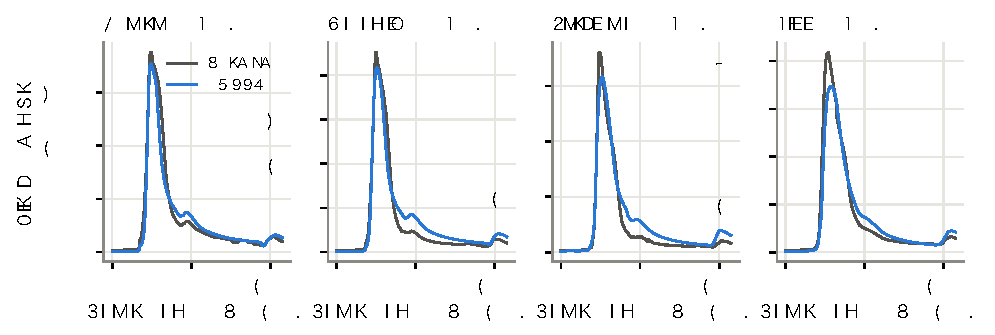
\includegraphics[width=\textwidth]{figs/v6_hydrographs.pdf}
\caption{Observed and 1K-RRI discharges of the 2019 flood (Typhoon Hagibis) at four gauges along the main river (a-priori parameters, no calibration).}
\label{fig:hydro}
\end{figure}

\paragraph{気候の与え方}
将来の降雨は、代表洪水の観測降雨 $r_i(t)$（セル $i$）を総雨量の倍率 $\alpha$ と強雨の強調 $\gamma$ で変換する:
\begin{equation}
r'_i(t)=c_i\,r_i(t)^{\gamma},\qquad \textstyle\sum_t r'_i(t)\,\Delta t=\alpha\sum_t r_i(t)\,\Delta t .
\label{eq:rain}
\end{equation}
海面上昇 $\Delta\eta$ は河口の潮位境界に加える。$\alpha$ の幅は治水計画の降雨量変化倍率\cite{mlit_teigen}、$\Delta\eta$ は日本の気候変動 2020\cite{jma2020}による（表\ref{tab:unc}）。

\subsection{被害額と浸水人口}
\label{sec:damage}
直接被害額は治水経済調査マニュアル（案）（令和 7 年 6 月改正, 令和 5 年評価額）\cite{mlit_manual}に従い、資産額と浸水深別の被害率の積の和とする:
\begin{equation}
D=\sum_{i}\Bigl[\sum_{c\in\mathcal{G}} V_{i,c}\,\rho_c\bigl(h_i-h^{f}_i;\,s_i\bigr)+V_{i,\mathrm{car}}\,\rho_{\mathrm{car}}(h_i)
+\sum_{c\in\{\text{水稲},\text{畑}\}} V_{i,c}\,\rho_c(h_i,\tau_i)\Bigr].
\label{eq:damage}
\end{equation}
$\mathcal{G}$ は家屋・家庭用品・事業所の償却資産と在庫・農漁家の償却資産と在庫、$h_i$ は最大浸水深、$h^f_i$ は床高（既定 0.45 m; 嵩上げで増える）、
$s_i$ は地盤勾配の群（A: $<1/1000$, B: $1/1000$〜$1/500$, C: $\ge1/500$; 1K-RRI の平野の平均勾配 $i_f$）、$\tau_i$ は浸水日数（浸水深 $\ge0.1$ m の時間 ÷ 24）である。
床上の被害率は床面からの浸水深を 0.5・1・2・3 m で区切った 5 区分、床下（$0<h<h^f$）は 1 区分とする（表\ref{tab:damrate}）。

$h_i$ は平野の最大水深 $h_f$（標高 $z_f$ が基準）である。1 km 格子のセル内では地盤高が大きく異なるため、セル内の 100 m 土地利用メッシュの地盤高（5 m 標高）の $z_f$ からの差の 20 分位 $z_{i,q}$ を
建物用地・農地ごとに保持し、セルの水量 $h_i A$ を全メッシュの標高分布に入れたときの水位 $H_i$ から、
分位ごとの浸水深 $h_{i,q}=\max(H_i-z_{i,q},0)$ で式(\ref{eq:damage})を評価して平均する（docs/03 §3.2-9）。

資産額 $V$ は、家屋＝延床面積 × 247.1 千円/m\textsuperscript{2}（福島県, 第 1 表）、家庭用品＝世帯数 × 9,368 千円、自動車＝世帯数 × 3,502 千円、
事業所＝産業大分類別の従業者数 × 第 3 表の単価、農漁家＝農家数 × 3,110（償却）・981（在庫）千円/戸、
水稲＝水田面積 × 532 kg/10a × 187 千円/t、畑作物＝畑面積 × 22.3 千円/a（令和 2 年の耕種−米の産出額 ÷ 畑面積）である。
世帯数・従業者数・農家数は国勢調査（250 m）・経済センサス（500 m）・農林業センサス（1 km）、土地利用は国土数値情報 L03-b\cite{ksj}による。

浸水人口は最大浸水深 0.5 m 以上のセルの人口 $P=\sum_i \mathrm{pop}_i\,\mathbf{1}(h_i\ge0.5\ \mathrm{m})$ とする。
2020〜2100 年の各評価年 $t$ では、代理モデルの予測に資産係数 $a(t)$・人口係数 $p(t)$（表\ref{tab:unc}; 2020 年から 2100 年まで線形）を掛ける:
$D_t=a(t)\,\hat D(\boldsymbol\phi_t)$、$P_t=p(t)\,\hat P(\boldsymbol\phi_t)$（\ref{sec:surrogate}節）。

\begin{table}[tbp]
\centering\footnotesize\setlength{\tabcolsep}{4pt}
\caption{Damage ratios (Manual for Economic Evaluation of Flood Control\cite{mlit_manual}, Tables 4.2--4.6)}
\label{tab:damrate}
\begin{tabular}{@{}lrrrrrr@{}}
\toprule
Asset (depth above floor) & Below floor & $<0.5$ m & 0.5--1 & 1--2 & 2--3 & $\ge3$ m \\
\midrule
House, group A (slope $<1/1000$) & 0.047 & 0.189 & 0.253 & 0.406 & 0.592 & 0.800 \\
House, group B ($1/1000$--$1/500$) & 0.058 & 0.219 & 0.301 & 0.468 & 0.657 & 0.843 \\
House, group C ($\ge1/500$) & 0.064 & 0.235 & 0.325 & 0.499 & 0.690 & 0.865 \\
Household goods & 0.037 & 0.308 & 0.533 & 0.701 & 0.948 & 0.977 \\
Business, depreciable & 0.064 & 0.296 & 0.573 & 0.801 & 0.920 & 0.940 \\
Business, inventory & 0.053 & 0.282 & 0.440 & 0.814 & 0.946 & 0.975 \\
Farm/fishery household, depreciable & 0 & 0.113 & 0.327 & 0.483 & 0.828 & 1.000 \\
Farm/fishery household, inventory & 0 & 0.223 & 0.584 & 0.618 & 0.792 & 0.942 \\
\bottomrule
\end{tabular}
\par\footnotesize\raggedright Cars (depth above ground): $<0.3$ m 0, 0.3--0.5 m 0.1, 0.5--0.7 m 0.5, $\ge0.7$ m 1.0.
Crops (depth × duration of 1--2/3--4/5--6/$\ge$7 days): rice $<0.5$ m 0.21/0.30/0.36/0.50, 0.5--1 m 0.24/0.44/0.50/0.71, $\ge1$ m 0.37/0.54/0.64/0.74;
upland crops (average) $<0.5$ m 0.27/0.42/0.54/0.67, 0.5--1 m 0.35/0.48/0.67/0.74, $\ge1$ m 0.51/0.67/0.81/0.91.
Sediment deposition ratios and the storey correction are not applied (no sediment model; no data on the mean number of storeys).
\end{table}



\subsection{年平均被害額（発生頻度に基づく便益）}
\label{sec:ead}
施策の便益は、治水経済調査マニュアル\cite{mlit_manual}の年平均被害軽減期待額に従い、確率規模 $T$ = 2, 5, 10, 20, 30, 50, 100, 150, 200 年の洪水の被害額 $D_T$ から
\begin{equation}
E=\sum_{j}\frac{D_{T_j}+D_{T_{j+1}}}{2}\Bigl(\frac{1}{T_j}-\frac{1}{T_{j+1}}\Bigr)
\label{eq:ead}
\end{equation}
とする（1/2 より頻繁な洪水と 1/200 より稀な洪水は数えない）。確率規模 $T$ の洪水は、代表洪水（1/100 とみなす, 仮定）の雨量を比 $r(T)$ と気候の降雨倍率 $\alpha$ で引き伸ばしたものとする:
$\alpha_T=\alpha\,r(T)$。$r(T)$ は流域内のアメダス 11 地点の年最大日降水量（43〜49 年）に地点ごとに L 積率法\cite{hosking1990}で Gumbel 分布を当てはめ、
$r(T)=x_T/x_{100}$ の中央値とした（表\ref{tab:freq}）。地点間の差は小さい（1/10 で 0.63〜0.70）。
仮定は、雨の時空間分布が代表洪水と同じであること、地点の日雨量の比で流域の雨量の比を代用すること、気候変動はすべての確率規模に同じ倍率で効くことである。

\begin{table}[tbp]
\centering\small
\caption{Rainfall ratio of the event of return period $T$ to the representative (1/100) event (Gumbel, L-moments, median of 11 AMeDAS stations)}
\label{tab:freq}
\begin{tabular}{@{}lrrrrrrrrr@{}}
\toprule
$T$ [yr] & 2 & 5 & 10 & 20 & 30 & 50 & 100 & 150 & 200 \\
$r(T)$ & 0.41 & 0.57 & 0.67 & 0.77 & 0.83 & 0.90 & 1.00 & 1.06 & 1.10 \\
\bottomrule
\end{tabular}
\end{table}

対策なし・現在気候の年平均被害額は 556 億円/年で、代表洪水 1 回 × 1/100（52 億円/年）の約 10 倍である（図\ref{fig:dfreq}）。
1/5 の洪水の被害額 866 億円・1/10 の 1,718 億円は大きく、低平地の小さな河道（断面は仮定）が中規模の洪水でもあふれる 1K-RRI の性質を反映している可能性がある（\ref{sec:limits}節）。

\begin{figure}[tbp]
\centering
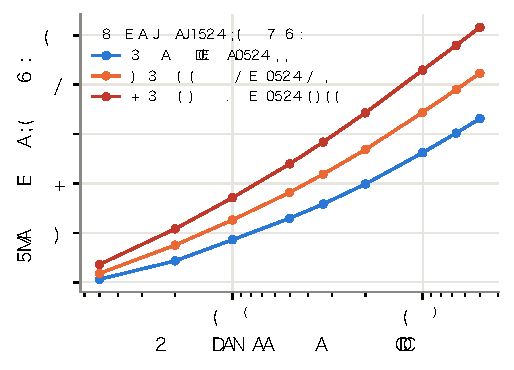
\includegraphics[width=0.55\textwidth]{figs/v6_damage_frequency.pdf}
\caption{Damage--frequency curves without measures (v6 surrogate) and the annual expected damage (EAD) for three climates.}
\label{fig:dfreq}
\end{figure}

\subsection{施策の表現}
\label{sec:meas-model}
各施策は 1K-RRI の入力（河道・土地利用クラス・資産・境界条件）の変更として表し、物理パラメータどおりに働く（効果係数は持たない）。
平野に働く施策（田んぼダム・排水ポンプ・貯留・移転・遊水地の用地）は平野の土地利用 $\mathrm{lc}_f$ に、森林整備は山地の土地利用 $\mathrm{lc}_s$ に作用する。
\begin{itemize}
  \item \textbf{堤防}: 河道の堤防高 $h_b\leftarrow h_b+\Delta H$（$\Delta H\in\{1,2\}$ m）。対象は集水面積 5 km\textsuperscript{2} 以上で、基準計算のピーク水位が天端 −0.2 m 以上の河道セル。
  \item \textbf{遊水地}: 計画中の阿武隈川上流遊水地群（350 ha・1,500 万 m\textsuperscript{3}\cite{mlit_usuichi}）。流入地点の流量のうち越流開始流量 $Q_c$ を超える分を取り込み、
    流量が $0.5Q_c$ を下回ってから排水する。$Q_c$ は基準計算でこの洪水が容量をちょうど満たす値（完全予見の運用）である。
  \item \textbf{田んぼダム}: 平野の土地利用が水田のセルの割合 $x$ で、地表水 0.15 m を保持し、満水時 5 mm/h で放流する\cite{maff_tanbo}。
  \item \textbf{森林整備}: 山地の森林の有効・不飽和間隙率を 20\% 増やす（土層厚は変えない; 仮定）。対象は山地のある全セルの割合 $x$。
    森林の洪水緩和機能は大規模洪水では限られるという評価\cite{scj2001,kuraji2004}があり、変化量は仮定である。
  \item \textbf{住宅の嵩上げ・移転}: 基準計算で浸水深 1 m 以上の世帯のあるセルで、床高を +1 m（嵩上げ）、または世帯・事業所を高台の新規造成地（HAND $>10$ m）へ移す（移転）。
  \item \textbf{排水ポンプ・排水機場}: 平野の地表水を本川側の河道へ 10 mm/h（市街地）・3 mm/h（農地）まで汲み上げる。
  \item \textbf{雨水貯留}: 市街地の平野に 30 mm（公共）・10 mm × 割合 $x$（各戸）の貯留を加え、満水時 2 mm/h で放流する。
\end{itemize}
単独の効果（他の施策なし）を表\ref{tab:v6measures}に示す。下流の堤防 +2 m（年平均被害額 −328 億円/年）、上流の田んぼダム（−195）、下流の移転（−381）の効果が大きい。

\begin{table}[tbp]
\centering\scriptsize\setlength{\tabcolsep}{2.5pt}
\caption{Single-measure effects (v6 surrogate, other measures absent; no effect coefficients). Costs [100 M JPY] from \texttt{costs.py}; change in the representative-event damage [100 M JPY] and the flooded population, and in the annual expected damage (EAD) [100 M JPY/yr]}
\label{tab:v6measures}
\begin{tabular}{@{}llrrrrrrr@{}}
\toprule
Measure & Level & Initial & Annual & $\Delta D$ current & $\Delta D$ 4\,\textdegree C & $\Delta$pop. current & $\Delta$EAD current & $\Delta$EAD 4\,\textdegree C \\
\midrule
Levee, up & +1 m & 295 & 0.0 & -8 & -153 & -2331 & -13 & -22 \\
Levee, up & +2 m & 548 & 0.0 & -13 & -301 & -4636 & -26 & -43 \\
Levee, mid & +1 m & 126 & 0.0 & -101 & -123 & -367 & 18 & 14 \\
Levee, mid & +2 m & 215 & 0.0 & -195 & -237 & -762 & 37 & 30 \\
Levee, down & +1 m & 372 & 0.0 & -1006 & -729 & -13750 & -203 & -403 \\
Levee, down & +2 m & 693 & 0.0 & -2002 & -2495 & -29505 & -328 & -708 \\
Retention basins, up & 350 ha, 15 Mm\textsuperscript{3} & 457 & 0.0 & -178 & -300 & -3442 & 55 & 65 \\
Paddy-field dam, up & 100\% & 18 & 1.4 & -1245 & -1370 & -12561 & -195 & -317 \\
Forest management, up & 100\% & 698 & 27.9 & -304 & -153 & -193 & -39 & -72 \\
Housing, up & raising +1 m & 56 & 0.0 & 59 & -60 & 2731 & -77 & -125 \\
Housing, up & relocation & 212 & 0.0 & -44 & -69 & -1079 & -61 & -94 \\
Paddy-field dam, mid & 100\% & 3 & 0.3 & -155 & -176 & -2217 & -26 & -51 \\
Forest management, mid & 100\% & 517 & 20.7 & -86 & -122 & 709 & -82 & -138 \\
Housing, mid & raising +1 m & 15 & 0.0 & -7 & -25 & -1154 & 2 & 2 \\
Housing, mid & relocation & 53 & 0.0 & 68 & -43 & -4361 & -6 & -1 \\
Paddy-field dam, down & 100\% & 9 & 0.7 & -66 & -261 & -865 & -48 & -83 \\
Forest management, down & 100\% & 633 & 25.3 & -233 & -77 & -1256 & -76 & -121 \\
Housing, down & raising +1 m & 693 & 0.0 & -1786 & -1981 & -45 & -189 & -349 \\
Housing, down & relocation & 2841 & 0.0 & -2888 & -3683 & -32105 & -381 & -754 \\
Urban pump, up & +10 mm/h & 97 & 1.9 & -31 & -39 & 1012 & -12 & -35 \\
Agri. pump, up & +3 mm/h & 138 & 2.8 & -12 & 40 & -983 & -28 & -33 \\
Public storage, up & 30 mm & 174 & 1.7 & 15 & -39 & -59 & 24 & 31 \\
Household storage, up & 100\% & 116 & 0.6 & 25 & -134 & 2052 & -5 & -18 \\
Urban pump, mid & +10 mm/h & 21 & 0.4 & -2 & 1 & -432 & 28 & 44 \\
Agri. pump, mid & +3 mm/h & 24 & 0.5 & 68 & -2 & 1154 & 4 & 13 \\
Public storage, mid & 30 mm & 38 & 0.4 & 12 & -38 & 797 & 46 & 73 \\
Household storage, mid & 100\% & 26 & 0.1 & 6 & -48 & -1535 & -27 & -46 \\
Urban pump, down & +10 mm/h & 327 & 6.5 & -19 & -104 & 772 & -10 & -8 \\
Agri. pump, down & +3 mm/h & 313 & 6.3 & -63 & 24 & -771 & -41 & -78 \\
Public storage, down & 30 mm & 588 & 5.9 & -45 & -28 & 1070 & -31 & -39 \\
Household storage, down & 100\% & 392 & 2.0 & 37 & -46 & -500 & -17 & -8 \\
\bottomrule
\end{tabular}
\par\footnotesize\raggedright Without measures: damage 5242 (current) / 8588 (4\,\textdegree C, rain ×1.2, sea level +0.70 m), flooded population 75135, EAD 556 / 1211. Positive $\Delta$EAD of some measures (retention basins, midstream levee, public storage) is an error of the surrogate for small floods (Section~\ref{sec:limits}).
\end{table}


\subsection{実施過程}
\label{sec:impl}
施策 $i$ が意思決定年 $t_d$ に水準 $x^{\mathrm{old}}\to x^{\mathrm{new}}$ へ変更されると、合意期間 $C$ の後に次の形で効果を持つ（\texttt{roadmap/sim.py}）:
\begin{align}
\text{(a) 堤防・遊水地}:&\quad x_i(t)=x^{\mathrm{old}}+(x^{\mathrm{new}}-x^{\mathrm{old}})\,\mathbf{1}(t\ge t_d+C+T_b),\\
\text{(b) その他}:&\quad x_i(t)=x^{\mathrm{old}}+(x^{\mathrm{new}}-x^{\mathrm{old}})\,\mathrm{clip}\Bigl(\frac{t-t_d-C}{T_b+T_u},0,1\Bigr).
\end{align}
(b) は住宅の嵩上げ・移転、排水ポンプ・排水機場、公共・各戸貯留、田んぼダム、森林整備、制度的施策で、施工・普及の期間 $T_b+T_u$ の間に効果が 0 → 100\% に線形に増える。
期間の名目値と範囲を表\ref{tab:unc}に示す。

\subsection{代理モデル}
\label{sec:surrogate}
代理モデルの入力は、施策の量（堤防の高さ/最大の高さ、遊水地の有無、実施率、嵩上げ・移転の割合）と気候の 3 変数（$\alpha$, $\Delta\eta$, $\gamma$; 探索範囲で $[0,1]$ に正規化）である。
出力ごとに $\log(1+D)$ 等を ARD 二乗指数カーネルのガウス過程\cite{rasmussen2006}で回帰し、リッジ回帰と一つ抜き交差検証の誤差で比べて良い方を使う。
学習点は、探索 v5（降雨倍率 1.0〜1.3; 施策・不確実性の LHS\cite{mckay1979} 320 点、対策なし 16 点、施策 1〜3 個の 80 点、目標の境界付近の適応追加 60 点）に、
v6 で降雨倍率 0.35〜1.5 の 160 点と対策なし 40 点を加えた 677 点である（RRI 計 707 回、検証を含む）。
検証（v6、30 点）は被害額 $R^2$ 1.00・相対 RMSE 8.0\%、浸水人口 0.97・16.9\% で、降雨倍率 1.0〜1.3 の被害額の誤差は 0.7\%、0.35〜0.7（小さな洪水, 平均 137 億円）は 30\% である。

\subsection{費用}
\label{sec:cost}
費用は施策の物理量 × 単価（表\ref{tab:unitcost}）で、現在価値は $C_{\mathrm{PV}}=C_0+C_a\sum_{y=1}^{50}1.04^{-y}$（年費用 $C_a$, 50 年・4\%）とする（表\ref{tab:v6measures}）。
実施モデルでは、初期費用を施工・普及の期間に配分し、維持費は毎年計上して 4\% で割り引く。
堤防の嵩上げは、天端幅 $b=5$ m・法勾配 $m=2$ の台形断面 $S(h)=h(b+mh)$ と敷幅 $W(h)=b+2mh$ から、
$C_0=L\{[S(h_0+\Delta H)-S(h_0)]c_{\mathrm{fill}}+c_{\mathrm{fix}}+[W(h_0+\Delta H)-W(h_0)]c_{\mathrm{land}}\}$（$L$: 両岸の延長、$h_0$: 既存の堤防高）とする。
遊水地は $C_0=V c_{\mathrm{exc}}+A c_{\mathrm{land}}+\sqrt{A}\,c_{\mathrm{weir}}+N_{\mathrm{hh}}c_{\mathrm{reloc}}$（$A$: 用地面積、越流堤長 $\sqrt{A}$）で、
上流遊水地群は 456.5 億円となる（1K-RRI の用地）。排水ポンプ・排水機場の能力は対象セルの面積 × 排水強度の和（m\textsuperscript{3}/s）である。

\begin{table}[tbp]
\centering\footnotesize
\caption{Unit costs (\texttt{costs.py}; assumed unless stated)}
\label{tab:unitcost}
\begin{tabularx}{\textwidth}{@{}l r L@{}}
\toprule
Item & Unit cost & Basis \\
\midrule
Levee fill $c_{\mathrm{fill}}$ / ancillary works $c_{\mathrm{fix}}$ & 8,000 JPY/m\textsuperscript{3} / 50,000 JPY/m & Excavation unit cost (319--777 JPY/m\textsuperscript{3}, design documents) plus material, haulage and compaction \\
Land $c_{\mathrm{land}}$ & 5,000 JPY/m\textsuperscript{2} & Typical price of rural farmland and forest \\
Retention excavation and embankment $c_{\mathrm{exc}}$ / weir $c_{\mathrm{weir}}$ & 1,500 JPY/m\textsuperscript{3} / 1 M JPY/m & As above plus haulage and disposal \\
Paddy-field dam boards / maintenance & 5,000 JPY/10a / 400 JPY/10a/yr & A few thousand JPY per board; paddy-field-dam subsidy of the multifunctional payment \\
Forest management (thinning, roads) / continuation & 0.5 M JPY/ha / 20 k JPY/ha/yr & Mountain area of the cells (1K-RRI $A_s$) \\
Relocation & 20 M JPY/household, 3 M JPY/employee & Group relocation projects, price-adjusted \\
House raising (floor) & 6 M JPY/household/m & House lifting \\
Drainage pump & 300 M JPY/(m\textsuperscript{3}/s), maintenance 2\%/yr & Typical cost of drainage pump stations \\
Rainwater storage public / household & 50 k / 100 k JPY/m\textsuperscript{3}, maintenance 500 JPY/m\textsuperscript{3}/yr & \\
\bottomrule
\end{tabularx}
\end{table}

%=====================================================================


%=====================================================================
\section{将来の不確実性と予測の学習}
\label{sec:uncertainty}

\subsection{真の将来と予測}
各評価シナリオ（世界）は、2100 年の降雨倍率 $X_r$ と海面上昇 $X_s$ の真値を持つ。真の経路は $\alpha(t)=1+(X_r-1)g_r(t)$、$\Delta\eta(t)=X_s g_s(t)$ で、
形 $g$ はすべての世界で共通である（2020 年 0、2050 年に降雨 0.6・海面 0.39、2100 年 1、その間は線形; 仮定）。
意思決定ルールは真値を知らず、各時点で得られる 2100 年の値の予測（平均 $m_t$、標準偏差 $s_t$）だけを使う。予測はガウス型の学習で表す:
事前分布は $N(\mu_0,\sigma_0^2)$（$\mu_0$: 計画時の想定 ×1.10・0.38 m、$\sigma_0$: 真値の範囲の (上限 − 下限)/$\sqrt{12}$）、
情報が $\mathrm{d}Y=X\,\mathrm{d}t+\kappa^{-1/2}\mathrm{d}W$ の形で連続的に入る（$W$ は世界ごとのブラウン運動）とすると、
\begin{equation}
m_t=\frac{\mu_0/\sigma_0^2+\kappa Y_t}{1/\sigma_0^2+\kappa(t-t_0)},\qquad s_t=\bigl(1/\sigma_0^2+\kappa(t-t_0)\bigr)^{-1/2}.
\label{eq:forecast}
\end{equation}
$m_t$ は（事前分布の下で）マルチンゲールで、真値に近づく。$\kappa$ は $s_t$ が半分になる年 $t_{1/2}$（学習の速さ, 2040〜2090 年; 仮定）から決める。
時点 $t$ から見た $h$ 年後の予測は $N(m_t,\,s_t^2-s_{t+h}^2)$ に従う（事前事後解析に使う）。観測誤差はない。

\subsection{評価シナリオ}
評価シナリオは、表\ref{tab:unc} の 3 群（気候・暴露・実施期間）の 14 因子を一様に振った LHS\cite{mckay1979} 256 標本である。ルールの探索には、別の乱数で作った探索シナリオ 64 標本を 3 組（seed）用いる。
Coverage は標本の割合であって、発生確率ではない。

\begin{table}[tbp]
\centering\small
\caption{Uncertain factors and ranges (docs/13 \texttt{world.py}; all assumed unless stated)}
\label{tab:unc}
\begin{tabularx}{\textwidth}{@{}>{\raggedright\arraybackslash}p{18mm} L >{\raggedright\arraybackslash}p{36mm} >{\raggedright\arraybackslash}p{22mm}@{}}
\toprule
Group & Factor & Range & Planner's value \\
\midrule
Climate & True rainfall factor in 2100 $X_r$ (MLIT: 2\,\textdegree C 1.1, 4\,\textdegree C 1.2) & 1.0--1.3 & prior mean 1.10 \\
 & True sea-level rise in 2100 $X_s$ (Tohoku: 2\,\textdegree C 0.38, 4\,\textdegree C 0.70 m) & 0.2--0.7 m & prior mean 0.38 m \\
 & Rainfall intensity exponent $\gamma$ & 0.9--1.2 & 1.0 \\
 & Year by which the forecast s.d. halves $t_{1/2}$ (learning speed) & 2040--2090 & 2060 \\
Exposure & Asset factor in 2100 (floodplain; linear from 2020) & 0.8--1.3 & 1.0 \\
 & Population factor in 2100 (floodplain; linear from 2020) & 0.6--1.05 & 0.8 \\
Durations & Levee / retention construction & 6--12 / 2--12 yr & 8 / 7 yr \\
 & Paddy-field dam / forest management diffusion & 4--19 / 5--20 yr & 9 / 10 yr \\
 & Housing (raising 3--18, relocation 2--17 yr), pumps and public storage (3--12 yr), household storage (5--20 yr) & Position in range 0--1 & 0.2--0.4 \\
\bottomrule
\end{tabularx}
\par\footnotesize Removed from the earlier model: effect coefficients and technology change, the year the climate departs from the planning path, the year assets start to change, observation errors.
\end{table}

%=====================================================================
\section{評価指標}
\label{sec:metrics}
\begin{itemize}
  \item \textbf{Target}: 2030 年から 5 年ごとの各評価期で、代表洪水の被害額 $\le$ 1.2 倍、浸水人口 $\le$ 1.5 倍（対策なし・現在気候に対して; 仮定）。
  \item \textbf{Target Coverage}: 評価シナリオのうち、2030〜2100 年のすべての評価期で Target を満たしたものの割合（最大化）。
  \item \textbf{累積費用}: 初期費用・維持費・変更費用の現在価値（割引率 4\%）の評価シナリオ平均（最小化）。
  \item \textbf{早い段階の備え}: 初期行動の初期費用。
\end{itemize}
残る将来の選択肢（Remaining Future Options）・Regret は用いない。単一の推奨は選ばず、Pareto front を示す。

%=====================================================================
\section{DAPP の作成方法}
\label{sec:method}

\subsection{全体の流れ}
\begin{figure}[tbp]
\centering
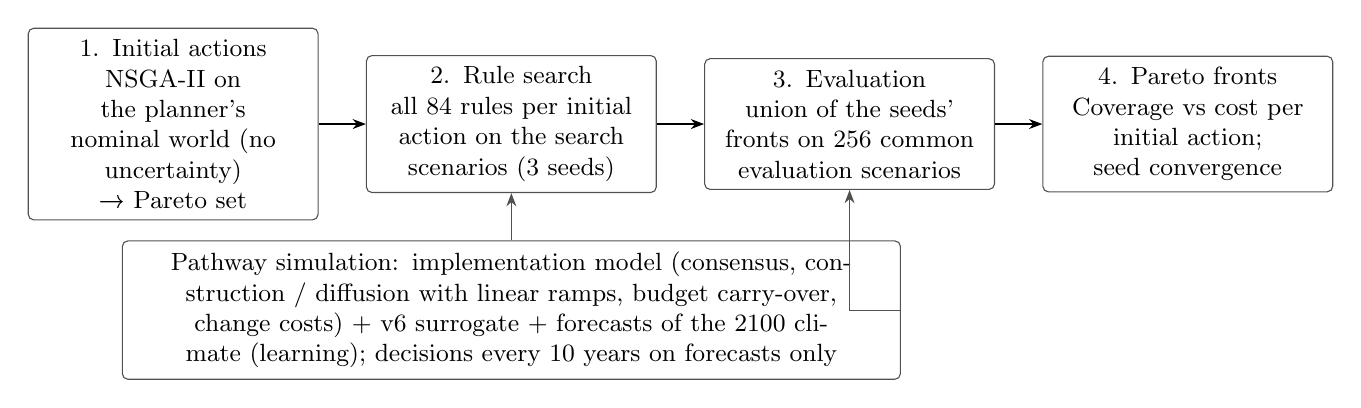
\begin{tikzpicture}[node distance=4mm and 6mm, every node/.style={font=\small}, box/.style={draw=cgray, rounded corners=2pt, align=center, inner sep=4pt, text width=34mm}]
\node[box] (a) {1. Initial actions\\NSGA-II on the planner's\\nominal world (no\\uncertainty) → Pareto set};
\node[box, right=of a] (b) {2. Rule search\\all 84 rules per initial\\action on the search\\scenarios (3 seeds)};
\node[box, right=of b] (c) {3. Evaluation\\union of the seeds'\\fronts on 256 common\\evaluation scenarios};
\node[box, right=of c] (d) {4. Pareto fronts\\Coverage vs cost per\\initial action;\\seed convergence};
\draw[-{Stealth}] (a) -- (b); \draw[-{Stealth}] (b) -- (c); \draw[-{Stealth}] (c) -- (d);
\node[box, below=6mm of b, text width=96mm] (e) {Pathway simulation: implementation model (consensus, construction / diffusion with linear ramps, budget carry-over, change costs) + v6 surrogate + forecasts of the 2100 climate (learning); decisions every 10 years on forecasts only};
\draw[-{Stealth}, cgray] (e) -- (b); \draw[-{Stealth}, cgray] (e.east) -| (c);
\end{tikzpicture}
\caption{Procedure of the Adaptive DAPP with forecasts and learning. No single recommendation is chosen.}
\label{fig:flow}
\end{figure}

\subsection{初期行動の候補}
計画者の標準値の世界（予測の事前分布の平均の気候経路、標準の実施期間、不確実性なし）で、施策の組合せを 2020 年から実施して何も加えない場合を評価する。
目的は初期費用・年平均被害額の現在価値・平均の浸水人口比の最小化で、初期費用 500 億円以下を制約として NSGA-II\cite{deb2002}（96 個体 × 80 世代）で探索した。
評価した 6,951 組合せのうち 177 が Pareto で、年平均被害額が最小のものから目的空間で互いに離れるように選んだ 14 個と施策なしを初期行動の候補とした（表\ref{tab:v6inits}）。

\begin{table}[tbp]
\centering\scriptsize\setlength{\tabcolsep}{2.4pt}
\caption{Composition of the 15 candidate initial actions (Pareto-efficient under the planner's nominal values; run \texttt{abukuma\_dapp\_forecast\_v6}). Levee: raised height [m]; paddy-field dam, forest management, household storage: implementation rate [\%]; housing: R = raising +1 m, M = relocation; \checkmark: built}
\label{tab:v6inits}
\begin{tabular}{@{}lccccccccccccccc@{}}
\toprule
Initial action & \#0 & \#1 & \#2 & \#3 & \#4 & \#5 & \#6 & \#7 & \#8 & \#9 & \#10 & \#11 & \#12 & \#13 & \#14 \\
Initial cost$^{\dagger}$ & 0 & 483 & 107 & 321 & 12 & 345 & 148 & 20 & 467 & 234 & 390 & 384 & 237 & 84 & 161 \\
EAD, PV$^{\dagger}$ (nominal) & 16.4k & 7.1k & 9.7k & 11.8k & 13.4k & 9.3k & 11.8k & 11.6k & 8.4k & 10.0k & 8.4k & 9.9k & 11.4k & 11.2k & 10.5k \\
\midrule
Levee, mid &  &  &  & +2 &  &  &  &  &  &  &  &  &  &  &  \\
Levee, down &  & +1 &  &  &  &  &  &  & +1 &  & +1 & +1 &  &  &  \\
Paddy-field dam, up &  & 100 & 100 & 100 & 50 & 100 & 100 & 100 & 100 & 100 & 100 & 50 & 100 & 100 & 100 \\
Housing, up &  & R & R &  &  & R &  &  &  & R &  &  &  &  & R \\
Paddy-field dam, mid &  & 100 & 100 & 100 & 100 & 100 & 100 & 50 & 100 & 100 &  & 100 & 100 & 100 & 100 \\
Forest management, mid &  &  &  &  &  & 50 &  &  &  &  &  &  &  &  &  \\
Housing, mid &  &  &  & M &  &  & M &  & M & M &  &  & M & M & M \\
Paddy-field dam, down &  & 100 & 50 &  &  & 100 &  &  &  & 50 &  &  &  &  &  \\
Household storage, up &  &  &  &  &  &  & 50 &  &  & 50 &  &  & 100 &  &  \\
Urban pump, mid &  &  &  & \checkmark &  &  & \checkmark &  & \checkmark & \checkmark &  &  & \checkmark &  & \checkmark \\
Household storage, mid &  & 100 & 100 & 50 &  &  &  &  &  & 100 &  &  & 100 & 50 & 50 \\
\bottomrule
\end{tabular}
\par\footnotesize\raggedright $^{\dagger}$100 M JPY. up/mid/down: upstream/midstream/downstream zone.
\end{table}


\subsection{意思決定ルール}
2030〜2090 年の 10 年ごとの意思決定時点で、次のルールに従う（表\ref{tab:policy}）。

\begin{table}[tbp]
\centering\small
\caption{Decision rule (all 84 combinations of the grid are evaluated)}
\label{tab:policy}
\begin{tabularx}{\textwidth}{@{}>{\raggedright\arraybackslash}p{24mm} L >{\raggedright\arraybackslash}p{30mm}@{}}
\toprule
Component & Content & Grid \\
\midrule
Monitoring & Forecast only: expected ratio $R_t$ of the committed portfolio at $t+L$, $R=\max(D/D^{*},P/P^{*})$ ($D^{*},P^{*}$: targets), expected over the forecast of the 2100 climate (3-point Gauss--Hermite on $N(m_t,s_t^2)$), exposure held at today's values & look-ahead $L\in\{10,20,30\}$ yr \\
Trigger & $R_t>\rho$ ($\rho$ × Target) & $\rho\in\{0.6,0.7,\dots,1.2\}$ \\
Choice & Among one-step upgrades that lower $R_t$ and fit the budget, those restoring $R_t\le1$; among them the largest net benefit $\mathrm{NB}_a=\mathrm{PV}\bigl(\Delta E\cdot\text{share in place}\bigr)-\mathrm{PV}(C_a)$, $E$: annual expected damage (Eq.~\ref{eq:ead}) expected over the forecast; if none restores it, the largest reduction of $R_t$. Lead times delay the benefit; no penalty terms & $k\in\{1,2\}$ actions per decision \\
Wait & Compare $\mathrm{NB}$ now with the value of deciding again after 10 years: $V_{\mathrm{wait}}=\delta^{10}\,\mathbb{E}_{m'}\bigl[\max(0,\max_a \mathrm{NB}_a(t+10\mid m'))\bigr]$, $m'\sim N(m_t,s_t^2-s_{t+10}^2)$; wait if $V_{\mathrm{wait}}>\mathrm{NB}$ and $R\le1$ at $t+10+$ the shortest lead time & on / off \\
\bottomrule
\end{tabularx}
\par\footnotesize Removed from the 11.11 rules: monitoring of observed damage and rainfall trends, cost / irreversibility / lead-time penalty weights, scale-back, remaining future options as an objective.
\end{table}

予算・リードタイム・変更費用は実施モデルが扱う（予算を超える行動は次の意思決定まで待つ）。計画者はルールの中で名目の実施期間を使う。

\subsection{探索と収束の確認}
初期行動ごとに 84 のルールすべてを、探索シナリオ 64 の 3 組（seed 11・12・13）で評価し、それぞれの Pareto front（Coverage 最大・累積費用最小）を得る。
3 組の front の和集合を共通の評価シナリオ 256 で評価し、その front を結果とする。収束は、各 seed の front の hypervolume と和集合の front の hypervolume の比（評価シナリオで）で確かめる。


%=====================================================================
\section{結果}
\label{sec:results}

\subsection{RQ1: 効率的な初期行動と適応ルール}
\begin{figure}[tbp]
\centering
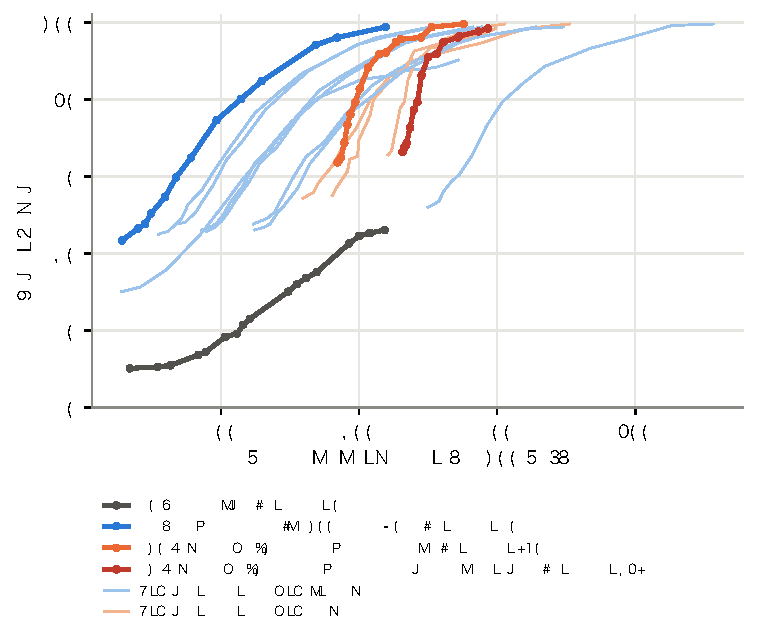
\includegraphics[width=0.72\textwidth]{figs/v6_fronts.pdf}
\caption{Pareto fronts (Target Coverage vs mean cumulative cost) of the decision rules for each of the 15 initial actions (256 evaluation scenarios). Thick lines: four representative initial actions (legend); thin lines: the other initial actions, without (blue) and with (orange) a levee in the initial action.}
\label{fig:fronts}
\end{figure}

\begin{table}[tbp]
\centering\small
\caption{Fronts of selected initial actions (256 evaluation scenarios; costs: mean cumulative cost, PV [100 M JPY]). HV ratio: minimum over the seeds of the hypervolume of a seed's front / that of the union}
\label{tab:fronts}
\resizebox{\textwidth}{!}{\begin{tabular}{@{}lrrrrrr@{}}
\toprule
Initial action & Initial cost & \multicolumn{2}{c}{Cheapest rule} & \multicolumn{2}{c}{Highest Coverage} & HV ratio \\
 & & Coverage & Cost & Coverage & Cost & \\
\midrule
\#0 No measures & 0 & 10\% & 68 & 46\% & 437 & 0.95 \\
\#4 Paddy-field dams (up 50\%, mid 100\%) & 12 & 30\% & 56 & 90\% & 543 & 0.99 \\
\#7 Paddy-field dams (up 100\%, mid 50\%) & 20 & 43\% & 56 & 99\% & 438 & 0.98 \\
\#13 Paddy-field dams, relocation mid, storage & 84 & 45\% & 109 & 99\% & 503 & 0.98 \\
\#2 Paddy-field dams, raising up, storage & 107 & 48\% & 135 & 99\% & 509 & 0.99 \\
\#10 Levee down +1 m, paddy-field dam up & 390 & 64\% & 369 & 100\% & 551 & 0.96 \\
\#8 Levee down +1 m, paddy-field dams, relocation mid, pumps & 467 & 66\% & 442 & 100\% & 611 & 0.98 \\
\#1 Levee down +1 m, paddy-field dams, raising up & 483 & 66\% & 463 & 98\% & 587 & 0.99 \\
\bottomrule
\end{tabular}}
\end{table}

\begin{figure}[tbp]
\centering
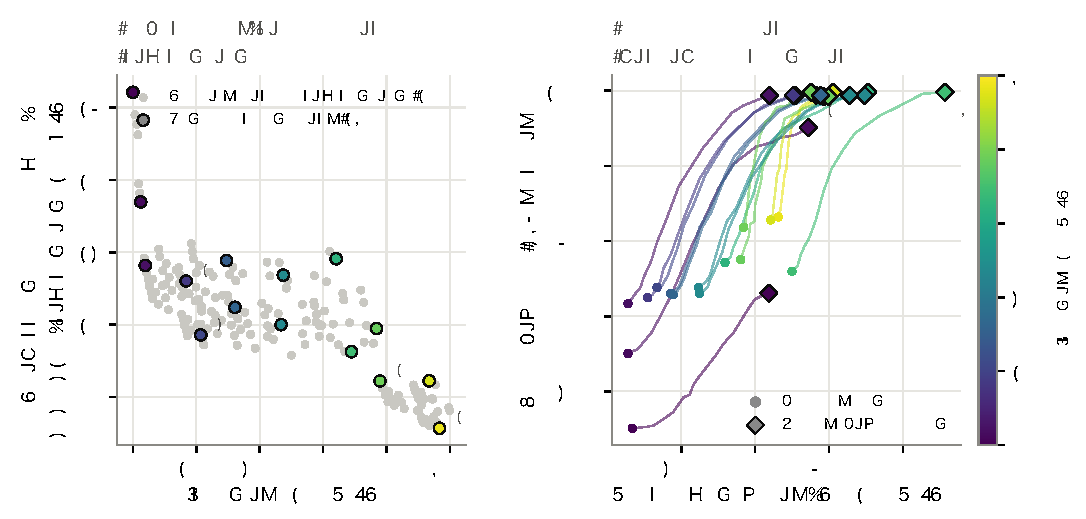
\includegraphics[width=\textwidth]{figs/v6_initial_actions.pdf}
\caption{Initial actions. (a) Pareto set of measure combinations on the planner's nominal world without adaptation (initial cost vs present value of the annual expected damage, 2020--2100) and the 15 selected initial actions. (b) The same initial actions with adaptation: Pareto front of the decision rules (lines), cheapest rule (circle) and highest-Coverage rule (diamond) (256 evaluation scenarios).}
\label{fig:inits}
\end{figure}

\begin{figure}[tbp]
\centering
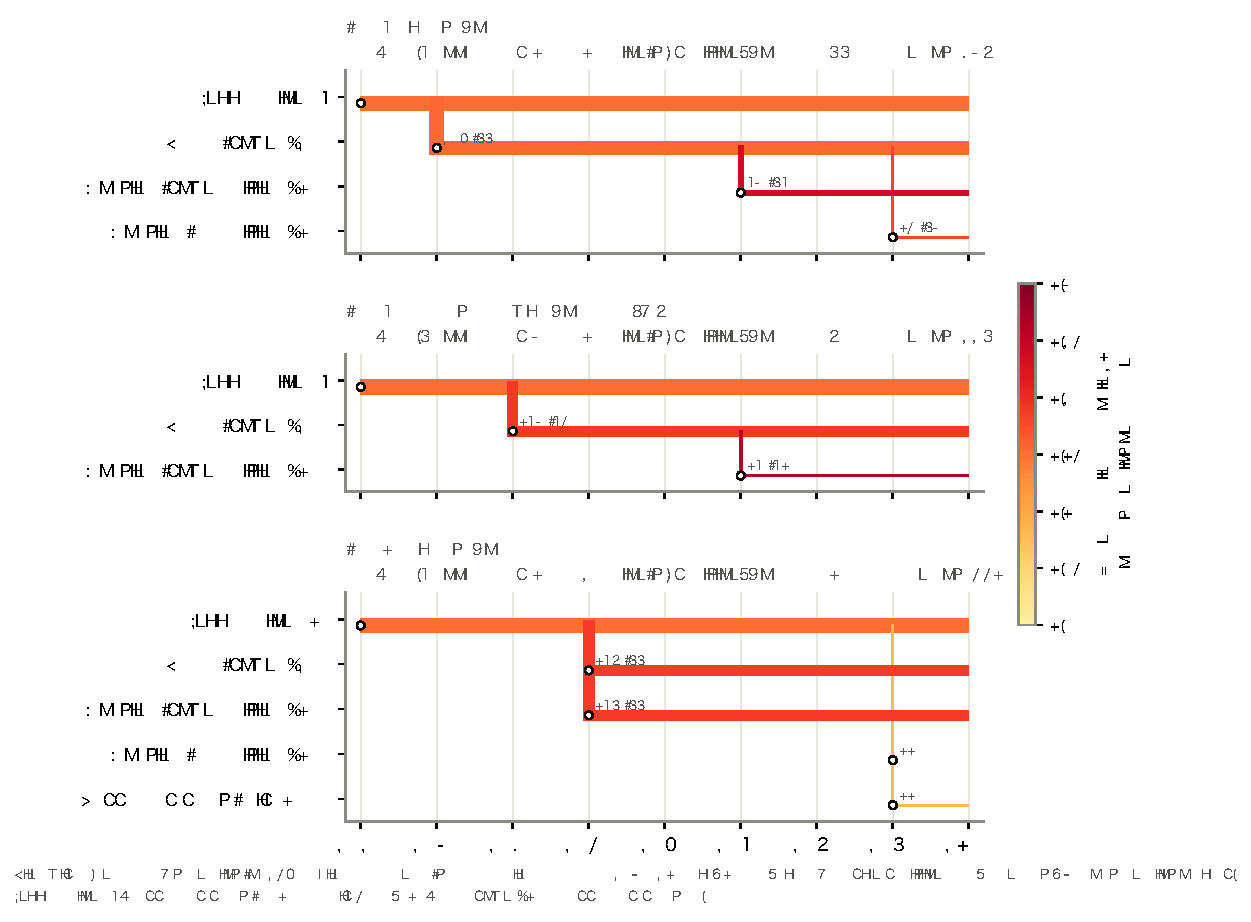
\includegraphics[width=0.98\textwidth]{figs/v6_pathways_map.pdf}
\caption{Adaptive Pathways Maps (DAPP) made by an initial action and a decision rule, built from the actions taken in the 256 evaluation scenarios: (a) initial action \#7 (paddy-field dams) with its highest-Coverage rule, (b) \#7 with the cheapest rule reaching Coverage 80\%, (c) \#10 (levee downstream +1 m, paddy-field dams) with its highest-Coverage rule. Each branch is a sequence of actions; colour: mean true rainfall factor in 2100 of the scenarios on the branch; numbers: scenarios on the branch and, if below 100\%, the share meeting the Target throughout.}
\label{fig:pathways}
\end{figure}

\begin{itemize}
  \item 施策なし（\#0）から始めると、最良のルール（$\rho$ 0.8、先読み 10 年、1 期 2 行動）でも Coverage は 46\%（費用 437 億円）である（図\ref{fig:fronts}、表\ref{tab:fronts}）。
    Target を最初に超えるのは 256 シナリオ中 134 が 2030 年代で、最初の意思決定（2030 年）で着手しても施策の完成（堤防 8 年など）が間に合わない。
    超えるかどうかは真の気候でほぼ決まる（2100 年の降雨倍率 1.0〜1.1 で 80\%、1.1〜1.2 で 44\%、1.2〜1.3 で 14\% が Target を満たす）。
  \item 田んぼダムだけの安い初期行動（\#7, 20 億円）から始め、$\rho$ 0.7・先読み 10 年のルールで適応すると、Coverage は 99\%、費用は 438 億円である。
    このルールは、最初の意思決定（2030 年）で 256 シナリオ中 201 で下流の堤防を加え、その後は下流の住宅対策を加える（図\ref{fig:actions}）。
    田んぼダムはすぐに被害を減らし、下流堤防が完成するまでの時間を稼ぐ。
  \item 下流堤防 +1 m を最初から含む初期行動（\#10・\#8・\#1; 390〜483 億円）は、最も安いルールでも Coverage 64〜66\% を保つ（早い段階の備え）。
    一方、Coverage 98〜100\% に要する平均累積費用は 551〜611 億円で、安い初期行動から適応する場合（438〜509 億円）より大きい。
    同じ Coverage を得るなら、初期に大きく投資するより、安い初期行動から予測に基づいて堤防を加える方が費用は小さい（図\ref{fig:time}）。
  \item 初期行動の分布（図\ref{fig:inits}）: 計画者の標準値の世界（適応なし）では、初期費用と年平均被害額の現在価値の間に明確なトレードオフがあり、堤防を含む候補（390〜483 億円）が被害額を最も小さくする（図\ref{fig:inits}(a)）。
    適応を加えると順位は変わり、初期費用の小さい田んぼダム中心の候補（\#7・\#13・\#2）が、同じ Coverage をより小さな累積費用で達成する（図\ref{fig:inits}(b)）。初期行動の評価は、その後の適応ルールと組で行う必要がある。
  \item 初期行動とルールが作る DAPP（図\ref{fig:pathways}）: \#7 に $\rho$ 0.7・先読み 10 年のルールを組み合わせると、ほぼすべてのシナリオ（246/256）が 2030 年頃に下流堤防 +2 m を加え、気候が厳しいシナリオ（73）は 2070 年頃に下流の住宅嵩上げを加える。
    同じ \#7 でも $\rho$ 0.9・先読み 30 年の安いルールでは、堤防の追加が 2040 年頃に遅れ（173 シナリオ）、Coverage は 80\%（累積費用 229 億円）に下がる。
    \#10 では堤防 +1 m が既にあるため、追加（+2 m と下流の住宅嵩上げ）は 2050 年頃まで遅らせられる。経路の分岐は少なく、主な違いは同じ施策を「いつ」加えるかである。住宅嵩上げを加える枝は真の降雨倍率が高いシナリオ（平均 1.2 以上）で、予測が気候の厳しさを捉えて枝分かれしている。Target を満たせないのは、この厳しい側の枝である（(b) で 71〜75\%）。
  \item 高い Coverage を与えるルールは、ほとんどが $\rho$ 0.7（Target の 0.7 倍で動く）・先読み 10 年である（15 の初期行動のうち 10）。
    Coverage の高い経路では、行動の 90\% が堤防・遊水地・住宅対策である。遊水地群は単独の効果の推定に誤差がある（表\ref{tab:v6measures}）ため選ばれにくい。
  \item 3 組の探索シナリオで得た front の hypervolume の比は 0.95〜0.99 で、全探索の結果はシナリオの組に対して安定している。
    ただし、front に入るルールの集合の重なりは 0.32〜0.73 で、front の近くには性能のほぼ等しいルールが並ぶ。
\end{itemize}

\begin{figure}[tbp]
\centering
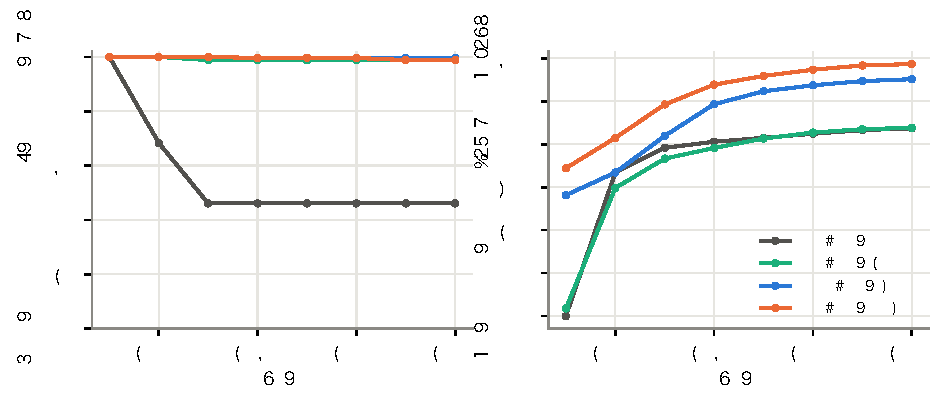
\includegraphics[width=0.98\textwidth]{figs/v6_time_course.pdf}
\caption{Share of scenarios meeting the Target up to each year and mean cumulative cost of the highest-Coverage rule of four initial actions (256 evaluation scenarios).}
\label{fig:time}
\end{figure}
\begin{figure}[tbp]
\centering
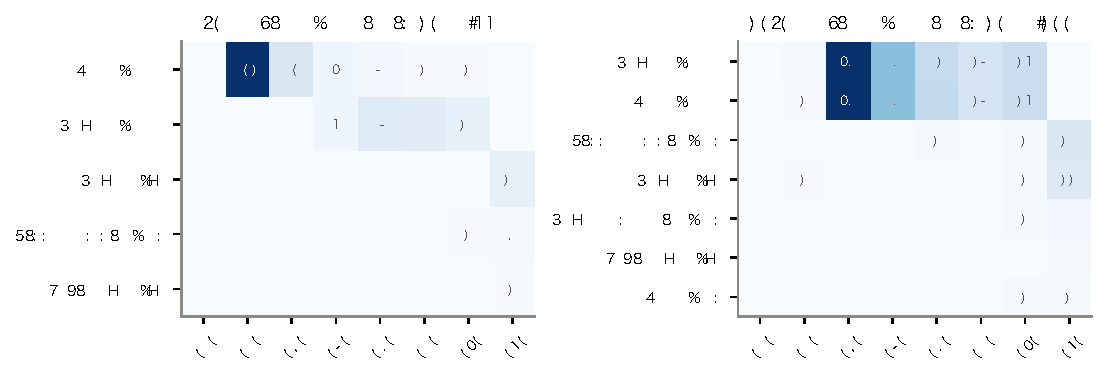
\includegraphics[width=0.98\textwidth]{figs/v6_actions.pdf}
\caption{Actions by measure and decision year (counts over the 256 evaluation scenarios) of the highest-Coverage rule of initial actions \#7 and \#10.}
\label{fig:actions}
\end{figure}

\subsection{RQ2: 今投資するか、情報を待つか}
\begin{itemize}
  \item 待つ判断を許すルールでも、待ったのは評価シナリオでの約 7.7 万回の判断のうち 22 回である。待つ判断の有無による Coverage の差は 0、費用の差は 0.2 億円である（全ルール平均）。
  \item 行動の 99\% は、そのときの予測で純便益が正である。年平均被害額の減少（下流堤防 +2 m で 328 億円/年）は施策の費用に比べて大きく、
    10 年待つと失われる便益が、待って得られる情報（予測の標準偏差の縮小）の価値を上回る。
  \item 予測の学習の速さは結果をほとんど変えない（\#7 の最良ルールで、予測の標準偏差が 2065 年より前に半分になるシナリオの Coverage 100\%、それ以降 98\%）。
    Target を超えるかどうかは、予測を待つことより、施策のリードタイムの間に被害を抑えられるか（早い段階の備え）で決まる。
  \item ただし、この結論は便益の大きさに依存する。頻度の高い洪水の被害が過大であれば（\ref{sec:limits}節）、純便益は小さくなり、待つ価値が相対的に大きくなる。
\end{itemize}

\subsection{RQ3: 計画時の想定と目標の水準}
\label{sec:rq3}
\begin{figure}[tbp]
\centering
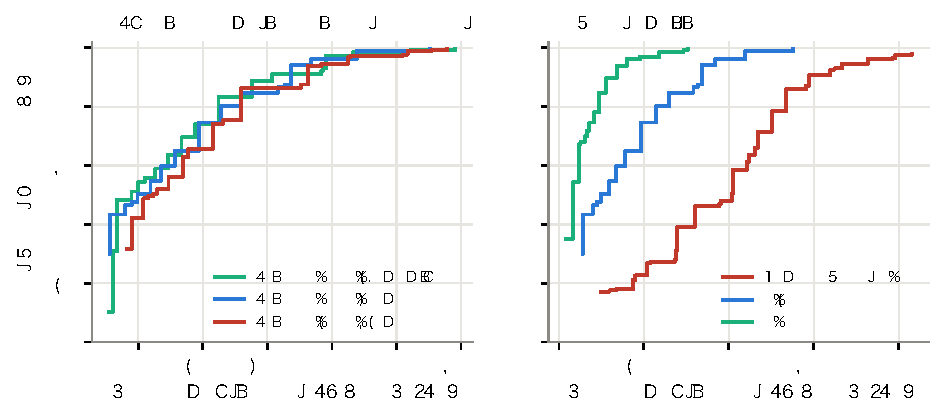
\includegraphics[width=0.98\textwidth]{figs/v6_sensitivity.pdf}
\caption{Best Target Coverage over all initial actions and rules against mean cumulative cost (256 evaluation scenarios). (a) Prior mean of the forecast (planning assumption); the true climates are the same. (b) Damage target (1.0, 1.2, 1.4 × the no-measure damage in the current climate).}
\label{fig:sens}
\end{figure}

\begin{table}[tbp]
\centering\small
\caption{Sensitivity to the planning assumption and the Target (256 evaluation scenarios; costs: mean cumulative cost, PV [100 M JPY]). ``Cheapest path to $\ge$98\%'': initial action with the lowest cost among the rules reaching Coverage $\ge$ 98\%}
\label{tab:sens}
\resizebox{\textwidth}{!}{\begin{tabular}{@{}lrrrrr@{}}
\toprule
Case & No measures & Paddy-field dams only & \multicolumn{2}{c}{Cheapest path to $\ge$98\%} & Levee in the initial action \\
 & max Coverage & max Coverage & Initial action (initial cost) & Cost & max Coverage (cost) \\
\midrule
Base (prior ×1.10, 0.38 m; Target 1.2) & 46\% & 99\% & Paddy-field dams (20) & 438 & 98--100\% (551--705) \\
Mild prior (×1.05, 0.29 m) & 46\% & 99\% & Paddy-field dams, raising, storage (112) & 512 & 98--100\% (522--663) \\
Severe prior (×1.25, 0.62 m) & 46\% & 91\% & Paddy-field dams, storage (56) & 517 & 98--100\% (556--578) \\
Target 1.0 & 4\% & 70\% & Levee down +1 m, paddy-field dams, raising, storage (483) & 831 & 92--98\% (800--888) \\
Target 1.4 & 94\% & 100\% & Paddy-field dams (20) & 236 & 98--100\% (432--518) \\
\bottomrule
\end{tabular}}
\par\footnotesize The initial actions are re-derived for each prior (the planner's nominal world changes); the Target cases use the base initial actions.
\end{table}

\begin{itemize}
  \item \textbf{計画時の想定（予測の事前分布）}: 事前分布の平均を ×1.05・0.29 m（穏やか）または ×1.25・0.62 m（厳しい）に変えても（真の気候は同じ）、
    Coverage と費用の関係はほとんど変わらない（図\ref{fig:sens}(a)）。施策なしの上限は 46\%、Coverage 98\% 以上に要する費用は 438〜517 億円である（表\ref{tab:sens}）。
    ルールは学習で更新される予測を監視するため、事前分布の偏りは意思決定の時点で多くが補正される。
  \item 想定が変えるのは初期行動の候補である（候補は計画者の標準値の世界で選ぶため）。堤防を含む候補は基準 5、穏やか 4、厳しい 3 で、厳しい想定では移転・各戸貯留・ポンプを多く含む候補が増える。
    どの想定でも、「安い初期行動から堤防を加える」経路と「堤防を最初に含む」経路の両方が Coverage 98\% 以上に達する。
  \item \textbf{Target の水準}: Target は結果を大きく変える（図\ref{fig:sens}(b)）。被害額 1.0 倍（現在の被害を増やさない）では、施策なしの Coverage は 4\%、田んぼダムだけから始めると 70\% が上限で、
    Coverage 90\% 以上に達するのは下流堤防 +1 m を最初から含む初期行動（\#1・\#8・\#10・\#11; 92〜98\%、費用 800〜888 億円）だけである。早い段階の備えが必要になる。
  \item 被害額 1.4 倍では、施策なしでも Coverage 94\% で、田んぼダム（\#7）から始めると 98\% を 236 億円で得る。堤防を最初に含む初期行動は 432〜518 億円で、安い初期行動の方が明らかに有利である。
  \item したがって、初期に大きく投資すべきかどうかは、気候の想定よりも Target の水準（どの被害の増加を許容するか）で決まる。
\end{itemize}


\subsection{RQ4: 便益の数え方}
\begin{figure}[tbp]
\centering
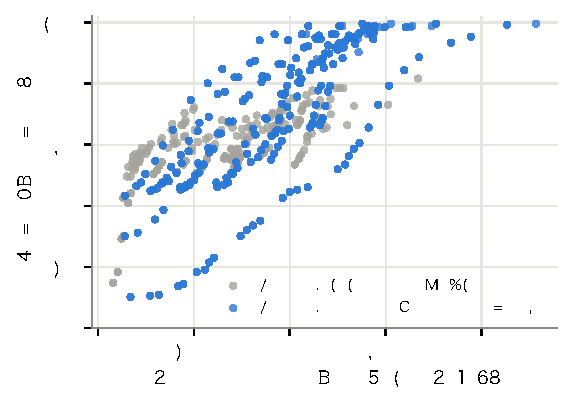
\includegraphics[width=0.6\textwidth]{figs/v6_valuation.pdf}
\caption{Pareto-front points of all initial actions with benefits counted as one representative event × 1/100 (explore v5, rule ``largest net benefit'') and as the annual expected damage (v6).}
\label{fig:valuation}
\end{figure}
\begin{itemize}
  \item 便益を代表洪水 1 回 × 1/100 で数えた計算（探索 v5、純便益が最大の行動を選ぶルール）では、純便益が最大の行動は田んぼダム・各戸貯留・排水ポンプに偏り、堤防は一度も選ばれなかった。
    Coverage の上限は 76\%（初期行動 \#1）である（図\ref{fig:valuation}）。
  \item 年平均被害額で数えると、純便益が最大の行動がそのまま Target を回復する行動にもなり、「目標を回復する行動のうち純便益最大」と「純便益最大」の二つの選び方の結果はほぼ一致した
    （行動の 99.7\% が予測した比を 1 以下に戻す）。
  \item 便益の数え方は、選ばれる施策の種類を変える。代表洪水 1 回の被害は、頻繁に起こる中小の洪水の被害を数えないため、大きな構造物の便益を過小に評価する。
\end{itemize}

%=====================================================================
\section{議論と限界}
\label{sec:limits}
\begin{itemize}
  \item \textbf{頻度の高い洪水の被害}: 対策なしの 1/5・1/10 の洪水の被害額（866・1,718 億円）は大きい。1K-RRI では低平地の小さな河道（断面は仮定、堤防なし）が中規模の洪水でもあふれる。
    阿武隈川の水害統計の年平均被害額と比べて確かめる必要がある。過大であれば、年平均被害額と便益が大きくなり、RQ2 の「待たない」結論を強めている可能性がある。
  \item \textbf{代理モデルの誤差}: 小さな洪水（降雨倍率 0.35〜0.7）の被害額の誤差は 30\% で、遊水地群・中流の堤防・公共貯留の単独の年平均被害額の変化は符号が逆になる（表\ref{tab:v6measures}）。
    遊水地群が選ばれにくいのはこの誤差による可能性がある。小さな洪水の学習点を増やす必要がある。
  \item \textbf{代表洪水と引き伸ばし}: 確率規模ごとの洪水は代表洪水の雨の時空間分布を引き伸ばしたもので、代表洪水を 1/100 とみなしている。複数の洪水波形での確認が必要である。
  \item \textbf{1K-RRI の仮定}: 論文にない仮定（表\ref{tab:k1assume}）のうち、河道の計算法（局所慣性式）と、河道でない代表セルの河道断面が結果に効きうる。パラメータは較正していない。
  \item \textbf{森林整備}: 間隙率 +20\% は仮定で、効果の範囲（不確実性）を持たない。
  \item \textbf{予測の学習}: 学習はガウス型の理想化で、予測の偏り（系統誤差）を含まない。経路の形 $g(t)$ は共通である。
  \item \textbf{扱わない過程}: 社会過程（合意の失敗・参加率）、評価基準の時間変化、施策の撤去・縮小。
\end{itemize}

%=====================================================================
\section{結論}
\begin{enumerate}
  \item 1K-RRI は 250 m モデルの流量と被害をよく再現し（NSE 0.90〜0.96、被害額 5,252 億円 / 7,452 億円）、1 km の計算で流域全体の施策の評価に使える。
  \item 施策なしから適応するだけでは、施策のリードタイムの間に Target を超えるシナリオ（2030 年代、約半数）を防げない。安くすぐ効く初期行動（田んぼダム）が、その間の被害を抑える。
  \item 安い初期行動から予測に基づいて堤防を加える経路は、初期に大きく投資する経路より安く、同等の Coverage（99\%）を得る。初期の大きな投資は、安いルールでも Coverage を保つ保険の役割を持つ。
  \item 便益を年平均被害額で数えると、Target を超えると予測された時点で行動する純便益は大きく、情報を待つ価値はほとんどない。代表洪水 1 回で数えると大きな構造物の便益を過小に評価する。
  \item 初期に大きく投資すべきかは、気候の想定（予測の事前分布）よりも Target の水準で決まる。現在の被害を増やさない Target では下流堤防を最初から含む初期行動が必要で、緩い Target では安い初期行動が有利である。
\end{enumerate}

%=====================================================================
\section{今後の計算と論文化の作業}
\label{sec:next}
\begin{itemize}
  \item 水害統計による年平均被害額の確認と、頻度の高い洪水の被害の検証（小さな河道の断面）。
  \item 小さな洪水の学習点を増やした代理モデル（遊水地群の評価）。
  \item 複数の洪水波形、予測の系統誤差、森林整備の効果の幅。
  \item RRI 本体による代表的な経路の状態の再計算（施策の配置と効果の地図）。
\end{itemize}

\subsection*{再現手順}
\begin{verbatim}
.venv/bin/python data/processed/explore/run_v5.py    # 1K-RRI, no effect coefficients
.venv/bin/python data/processed/explore/run_v6.py    # + events of other return periods
.venv/bin/python scripts/run_roadmap.py --prepare     # cost table (physics.explore_run)
.venv/bin/python scripts/run_forecast_dapp.py         # abukuma_dapp_forecast_v6
.venv/bin/python docs/paper/dapp/measure_effects_v6.py
.venv/bin/python docs/paper/dapp/make_figs_v6.py
\end{verbatim}

\begin{thebibliography}{99}\small
\bibitem{sugawara2024} 菅原快斗・佐山敬洋・山田真史・山本浩大 (2024): 広域かつ高速な降雨流出氾濫計算のためのマクロスケール RRI モデルの開発, 土木学会論文集, 80(16), 23-16125.
\bibitem{tachikawa2004} 立川康人・永谷言・寶馨 (2004): 飽和・不飽和流れの機構を導入した流量流積関係式の開発, 水工学論文集, 48, 7--12.
\bibitem{masutani2006} 舛谷敬一・赤井計之・馬籠純 (2006): 格子状擬河道網のスケール変換に関する新しい方法, 水文・水資源学会誌, 19(2), 139--150.
\bibitem{hosking1990} Hosking, J.R.M. (1990): L-moments: analysis and estimation of distributions using linear combinations of order statistics, \textit{Journal of the Royal Statistical Society B}, 52(1), 105--124.
\bibitem{dixit1994} Dixit, A.K., Pindyck, R.S. (1994): \textit{Investment under Uncertainty}, Princeton University Press.
\bibitem{raiffa1961} Raiffa, H., Schlaifer, R. (1961): \textit{Applied Statistical Decision Theory}, Harvard University.
\bibitem{sayama2012} Sayama, T., Ozawa, G., Kawakami, T., Nabesaka, S., Fukami, K. (2012): Rainfall–runoff–inundation analysis of the 2010 Pakistan flood in the Kabul River basin, \textit{Hydrological Sciences Journal}, 57(2), 298--312.
\bibitem{bates2010} Bates, P.D., Horritt, M.S., Fewtrell, T.J. (2010): A simple inertial formulation of the shallow water equations for efficient two-dimensional flood inundation modelling, \textit{Journal of Hydrology}, 387(1--2), 33--45.
\bibitem{greenampt1911} Green, W.H., Ampt, G.A. (1911): Studies on soil physics, Part I: The flow of air and water through soils, \textit{Journal of Agricultural Science}, 4(1), 1--24.
\bibitem{honma1940} 本間仁 (1940): 低溢流堰堤の流量係数, 土木学会誌, 26(6), 635--645; 26(9), 849--862.
\bibitem{renno2008} Rennó, C.D., Nobre, A.D., Cuartas, L.A., et al. (2008): HAND, a new terrain descriptor using SRTM-DEM: Mapping terra-firme rainforest environments in Amazonia, \textit{Remote Sensing of Environment}, 112(9), 3469--3481.
\bibitem{nobre2011} Nobre, A.D., Cuartas, L.A., Hodnett, M., et al. (2011): Height Above the Nearest Drainage -- a hydrologically relevant new terrain model, \textit{Journal of Hydrology}, 404(1--2), 13--29.
\bibitem{mlit_manual} 国土交通省 水管理・国土保全局 (2025): 治水経済調査マニュアル（案）（令和 7 年 6 月改正）.
\bibitem{mlit_usuichi} 国土交通省 東北地方整備局 福島河川国道事務所: 阿武隈川上流遊水地群の概要, \url{https://www.thr.mlit.go.jp/fukushima/usuichi_faq/1-1-1_sisetugaiyou.pdf}（2026 年 11 月閲覧）.
\bibitem{mlit_teigen} 気候変動を踏まえた治水計画に係る技術検討会 (2021): 気候変動を踏まえた治水計画のあり方 提言（改訂版）, 国土交通省.
\bibitem{mlit_ryuiki} 社会資本整備審議会 (2020): 気候変動を踏まえた水災害対策のあり方について ～あらゆる関係者が流域全体で行う持続可能な「流域治水」への転換～（答申）.
\bibitem{jma2020} 文部科学省・気象庁 (2020): 日本の気候変動 2020 －大気と陸・海洋に関する観測・予測評価報告書－.
\bibitem{maff_tanbo} 農林水産省 農村振興局 (2022): 「田んぼダム」の手引き.
\bibitem{scj2001} 日本学術会議 (2001): 地球環境・人間生活にかかわる農業及び森林の多面的な機能の評価について（答申）.
\bibitem{kuraji2004} 蔵治光一郎・保屋野初子 編 (2004): 緑のダム ―森林・河川・水循環・防災―, 築地書館.
\bibitem{ksj} 国土交通省: 国土数値情報（土地利用細分メッシュ L03-b、行政区域 N03、国有林野 A45）.
\bibitem{haasnoot2013} Haasnoot, M., Kwakkel, J.H., Walker, W.E., ter Maat, J. (2013): Dynamic adaptive policy pathways: A method for crafting robust decisions for a deeply uncertain world, \textit{Global Environmental Change}, 23(2), 485--498.
\bibitem{kwadijk2010} Kwadijk, J.C.J., Haasnoot, M., Mulder, J.P.M., et al. (2010): Using adaptation tipping points to prepare for climate change and sea level rise: a case study in the Netherlands, \textit{WIREs Climate Change}, 1(5), 729--740.
\bibitem{lempert2003} Lempert, R.J., Popper, S.W., Bankes, S.C. (2003): \textit{Shaping the Next One Hundred Years: New Methods for Quantitative, Long-Term Policy Analysis}, RAND, MR-1626.
\bibitem{kwakkel2016} Kwakkel, J.H., Haasnoot, M., Walker, W.E. (2016): Comparing Robust Decision-Making and Dynamic Adaptive Policy Pathways for model-based decision support under deep uncertainty, \textit{Environmental Modelling \& Software}, 86, 168--183.
\bibitem{giuliani2016} Giuliani, M., Castelletti, A., Pianosi, F., Mason, E., Reed, P.M. (2016): Curses, tradeoffs, and scalable management: Advancing evolutionary multiobjective direct policy search to improve water reservoir operations, \textit{Journal of Water Resources Planning and Management}, 142(2), 04015050.
\bibitem{quinn2017} Quinn, J.D., Reed, P.M., Keller, K. (2017): Direct policy search for robust multi-objective management of deeply uncertain socio-ecological tipping points, \textit{Environmental Modelling \& Software}, 92, 125--141.
\bibitem{haasnoot2018} Haasnoot, M., van 't Klooster, S., van Alphen, J. (2018): Designing a monitoring system to detect signals to adapt to uncertain climate change, \textit{Global Environmental Change}, 52, 273--285.
\bibitem{hermans2017} Hermans, L.M., Haasnoot, M., ter Maat, J., Kwakkel, J.H. (2017): Designing monitoring arrangements for collaborative learning about adaptation pathways, \textit{Environmental Science \& Policy}, 69, 29--38.
\bibitem{deb2002} Deb, K., Pratap, A., Agarwal, S., Meyarivan, T. (2002): A fast and elitist multiobjective genetic algorithm: NSGA-II, \textit{IEEE Transactions on Evolutionary Computation}, 6(2), 182--197.
\bibitem{mckay1979} McKay, M.D., Beckman, R.J., Conover, W.J. (1979): A comparison of three methods for selecting values of input variables in the analysis of output from a computer code, \textit{Technometrics}, 21(2), 239--245.
\bibitem{rasmussen2006} Rasmussen, C.E., Williams, C.K.I. (2006): \textit{Gaussian Processes for Machine Learning}, MIT Press.
\end{thebibliography}


\end{document}
